\documentclass{article}
%documentclass[draft]{article}

\usepackage[italian]{babel}
\usepackage[utf8]{inputenc}


\usepackage{graphicx} % Immagini fantastiche e...
\graphicspath{        % dove trovarle
  {./images/},
}

%%% Bibliografia
%\usepackage{csquotes}
%\usepackage{biblatex}
%\addbibresource{bibl.bib}


% Grafici direttamente in latex
\usepackage{tikz}
\usetikzlibrary{shapes,positioning,calc}
\colorlet{lightgray}{gray!20}

\usepackage{rotating} % per tabella ruotata
\usepackage{makecell}
%\usepackage[showframe=true]{geometry}
\usepackage{changepage}

% Immagini galleggiano
\usepackage{float}

\usepackage{color}

\usepackage{caption}
% per caption ad immagini in tab annidiate
\usepackage{subcaption}

\usepackage{hyperref} % lasciare per ultimo
%\hypersetup{colorlinks=true, linkcolor=blue, citecolor=black, plainpages=false, urlcolor=blue}
\hypersetup{colorlinks=true, linkcolor=black, citecolor=black, plainpages=false, urlcolor=blue}

% Usato nella copertina
\usepackage{wallpaper}



\usepackage{listings}
\lstset{
  showspaces=false,
  showstringspaces=false,
  basicstyle=\ttfamily,
  %numbers=left,
  %numbers=none,
  numberstyle=\small,
  mathescape
}

\usepackage{algpseudocode,algorithm,algorithmicx}


% Simboli matematici
%\usepackage{amsthm}
\usepackage{amssymb}
\usepackage{amsmath}
%\usepackage{amsfonts}
%\usepackage{mathabx} % per \topdoteq
%\usepackage{mathtools, amsthm}


% Comodo per evidenziare zone da modificare
\usepackage{todonotes} 

% Lorem ipsum...
\usepackage{lipsum} 


 
% ================================ %
%          Cose Personali          %
% ================================ %

% Alcune comodita' logico/matematiche
\let\ep\epsilon
\let\b\bullet
\let\iff\Leftrightarrow
\newcommand{\viff}{\Updownarrow}
\let\impl\Rightarrow

\newcommand{\norm}[1]{\lvert\lvert #1 \lvert\lvert}
\newcommand{\Norm}[1]{\Big\lvert \Big\lvert #1 \Big\lvert \Big\lvert}

\newcommand\N{\ensuremath{\mathbb{N}}}
\newcommand\R{\ensuremath{\mathbb{R}}}
\newcommand\Z{\ensuremath{\mathbb{Z}}}
\renewcommand\O{\ensuremath{\emptyset}}
\newcommand\Q{\ensuremath{\mathbb{Q}}}
\newcommand\C{\ensuremath{\mathbb{C}}}

\newcommand\E{\ensuremath{\mathbb{E}}}
\newcommand\T{\ensuremath{\mathbb{T}}}
\renewcommand\inf{\ensuremath{\infty}}




% ================================ %
%            Il Documento          %
% ================================ %
\begin{document}

% ================================ %
%        Creo Prima Pagina         %
% ================================ %

\ThisCenterWallPaper{0.95}{polloPallido}
% Intestazione
% TODO Migliorare esteticamente
\begin{titlepage}
 	\centering
  \Huge{\textbf{Progetto Ragionamento Automatico}}\\
 	[30mm]
 	\centering
  \Huge{\textbf{Studente: Tristano Munini}}\\
 	%[25mm]
  %\raggedright
  %\Large{\textbf{Corso:}}\\
  %\Large{\textbf{TODO}}\\
 	[125mm]
 	\centering
  \LARGE{\underline{\textbf{ANNO ACCADEMICO 2019-2020}}}\\
\end{titlepage}

%% ================================ %
%%              Indice              %
%% ================================ %
%\tableofcontents
%\thispagestyle{empty}
%\cleardoublepage
%\setcounter{page}{1}


% ================================ %
%      Qua Inizia La Tesina        %
% ================================ %
%\abstract{
%  \lipsum[1]
%}

%\pagenumbering{gobble} % TODO REMOVE


%!TEX TS-program = pdflatex
%!TEX root = main.tex
%!TEX encoding = UTF-8 Unicode

\section{Il problema}
Si riporta il testo della consegna
\begin{figure}[ht]
  \centering
  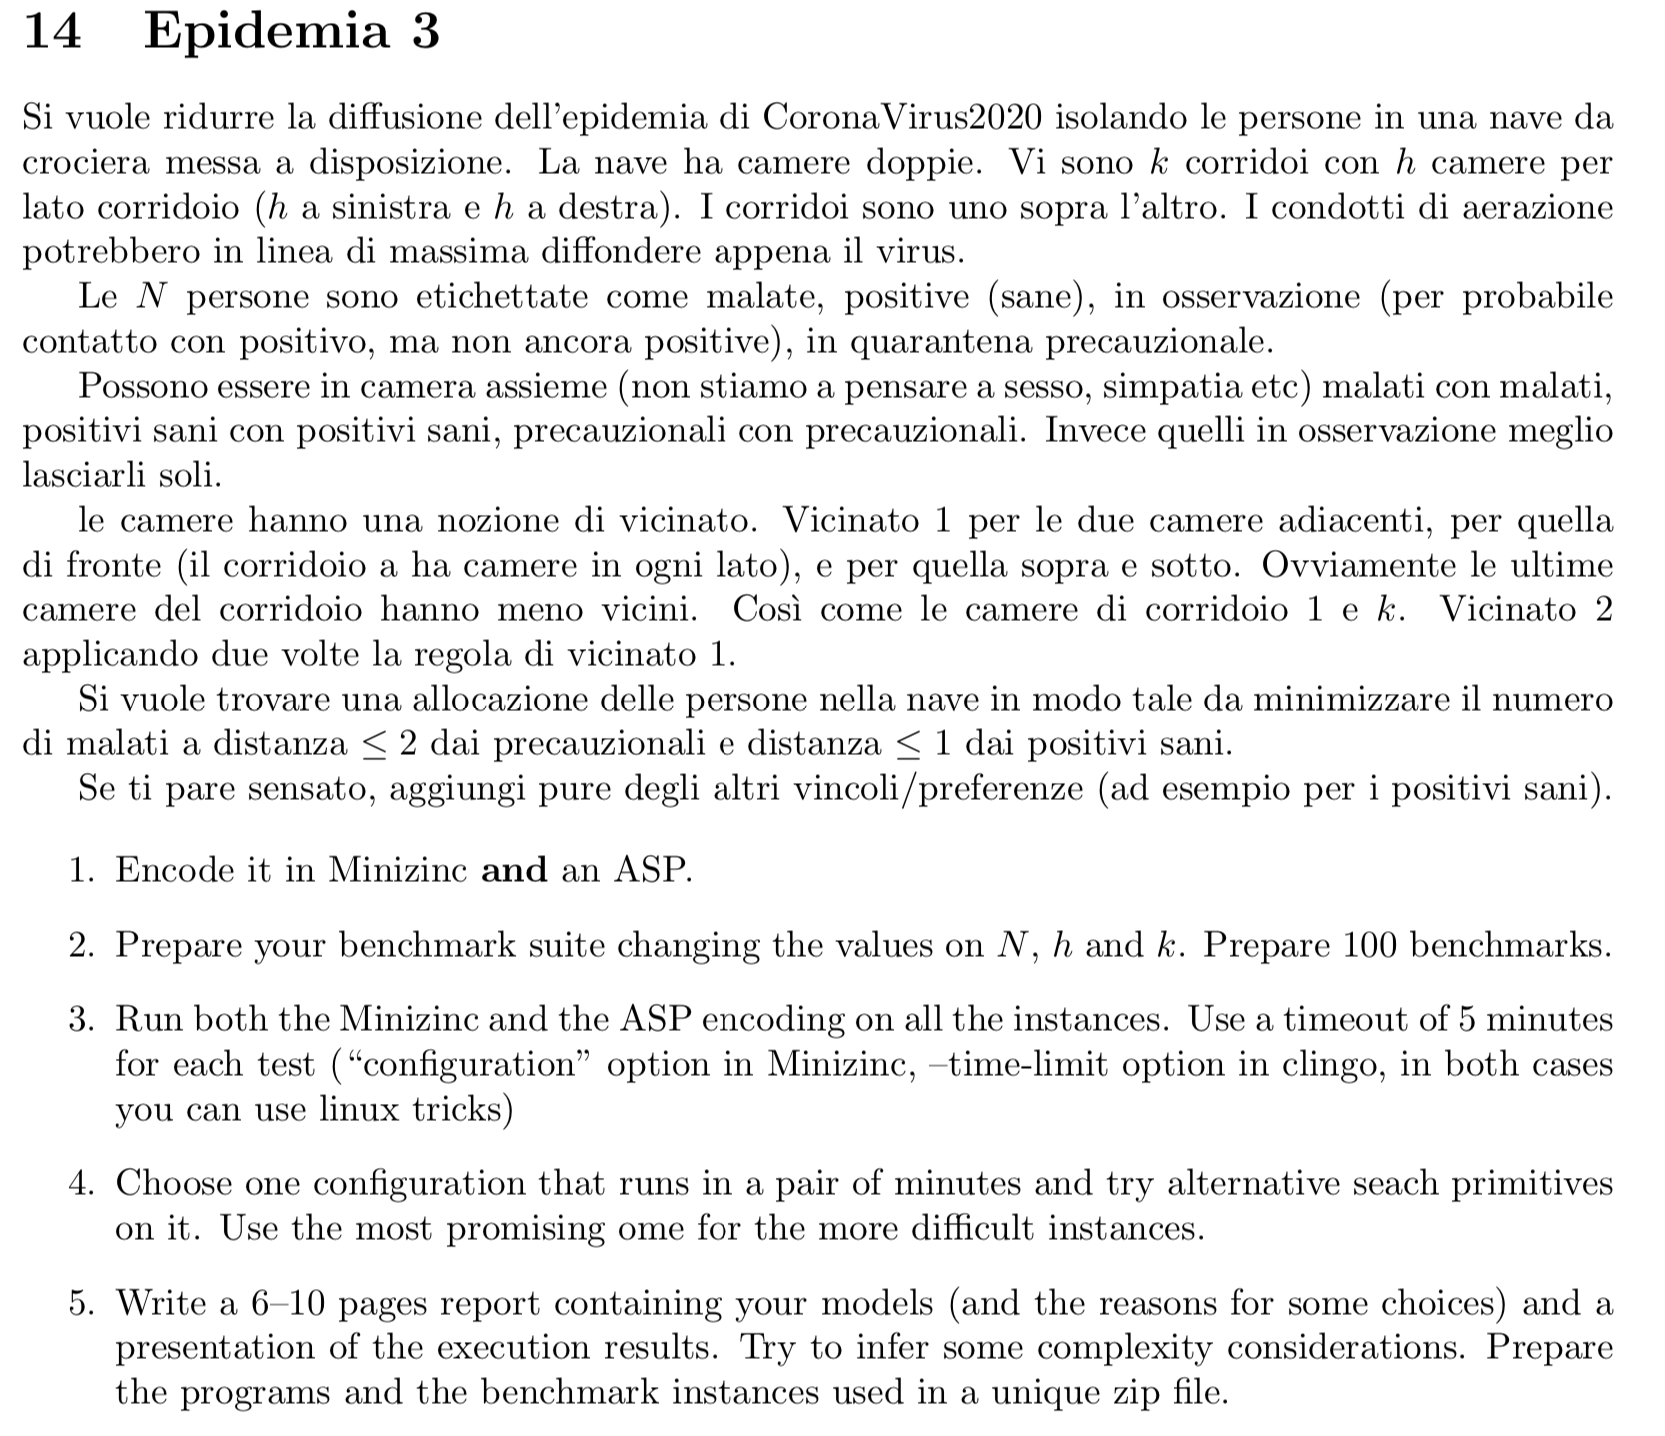
\includegraphics[width=\textwidth]{MUNINI}
\end{figure}


%% ================================ %
%%           Bibliografia           %
%% ================================ %
%%\cleardoublepage
%%\printbibliography

\end{document}
